\documentclass[11pt]{amsart}
\usepackage[utf8]{inputenc}
\usepackage[english]{babel}
\usepackage{amsmath}
\usepackage{amsfonts}
\usepackage{amssymb}
\usepackage[all]{xy}
\usepackage{graphicx}
\usepackage{xcolor}

\begin{document}

\title{Modelling Stochastic Time Delay Structures for Regression}
\author{Aaron Pickering}
%\address{}
\email{aaron1rcl@gmail.com}
%\urladdr{} 
\date{\today}
\maketitle

\section{Introduction}

Consider the typical univariate regression problem where the intention is to find the relationship between $x$ and $y$. When extended to time series, a number of time specific complexities arise. For the specific case where the input $x$ affects the output $y$, with a random time delay in between, the estimated coefficients (or weights, predictions etc) are significantly attenuated. This attenuation occurs both in traditional statistical models and machine learning models, and for certain problems can be a serious limitation. The following document proposes techniques for handling this class of time series regression.

As an example, let us take the management of blood sugar level in diabetes patients. In people with diabetes, the pancreas can't effectively regulate blood sugar levels. Therefore, these levels must be controlled by insulin injections and a special diet. The challenge for many people is that the relationship between the input (insulin) and output (blood sugar) is extremely complex. The effect of the insulin injection might be observed after $15$, $20$  or $t$ minutes depending on a number of factors, many of which are unknown. Due to the stochastic nature of the time delays, the actual effect can't be easily determined. It is difficult to differentiate the effect of the insulin injection from other factors and accurately determine how much one should take.

Inference for this type of problem is especially challenging. Typical regression models require a fixed alignment between cause and effect. Using standard methods, we'd need to assume that the effect occurs after some fixed time $t$ which can be inferred from the data. However, if there is any uncertainty in the parameter $t$ ($t$ changes or is noisy) the resulting estimates will be significantly attenuated.

Consider the simple example where the effect of the input is $1$, as shown in the image below. The observed input is given by the red line, the blue line is when the effect actually occurs. The first effect happens one time point after the input. The second effect happens at the same time as the input. A fixed time delay isn't valid in this case because the time shifts differ.

\begin{center}
\begin{figure}
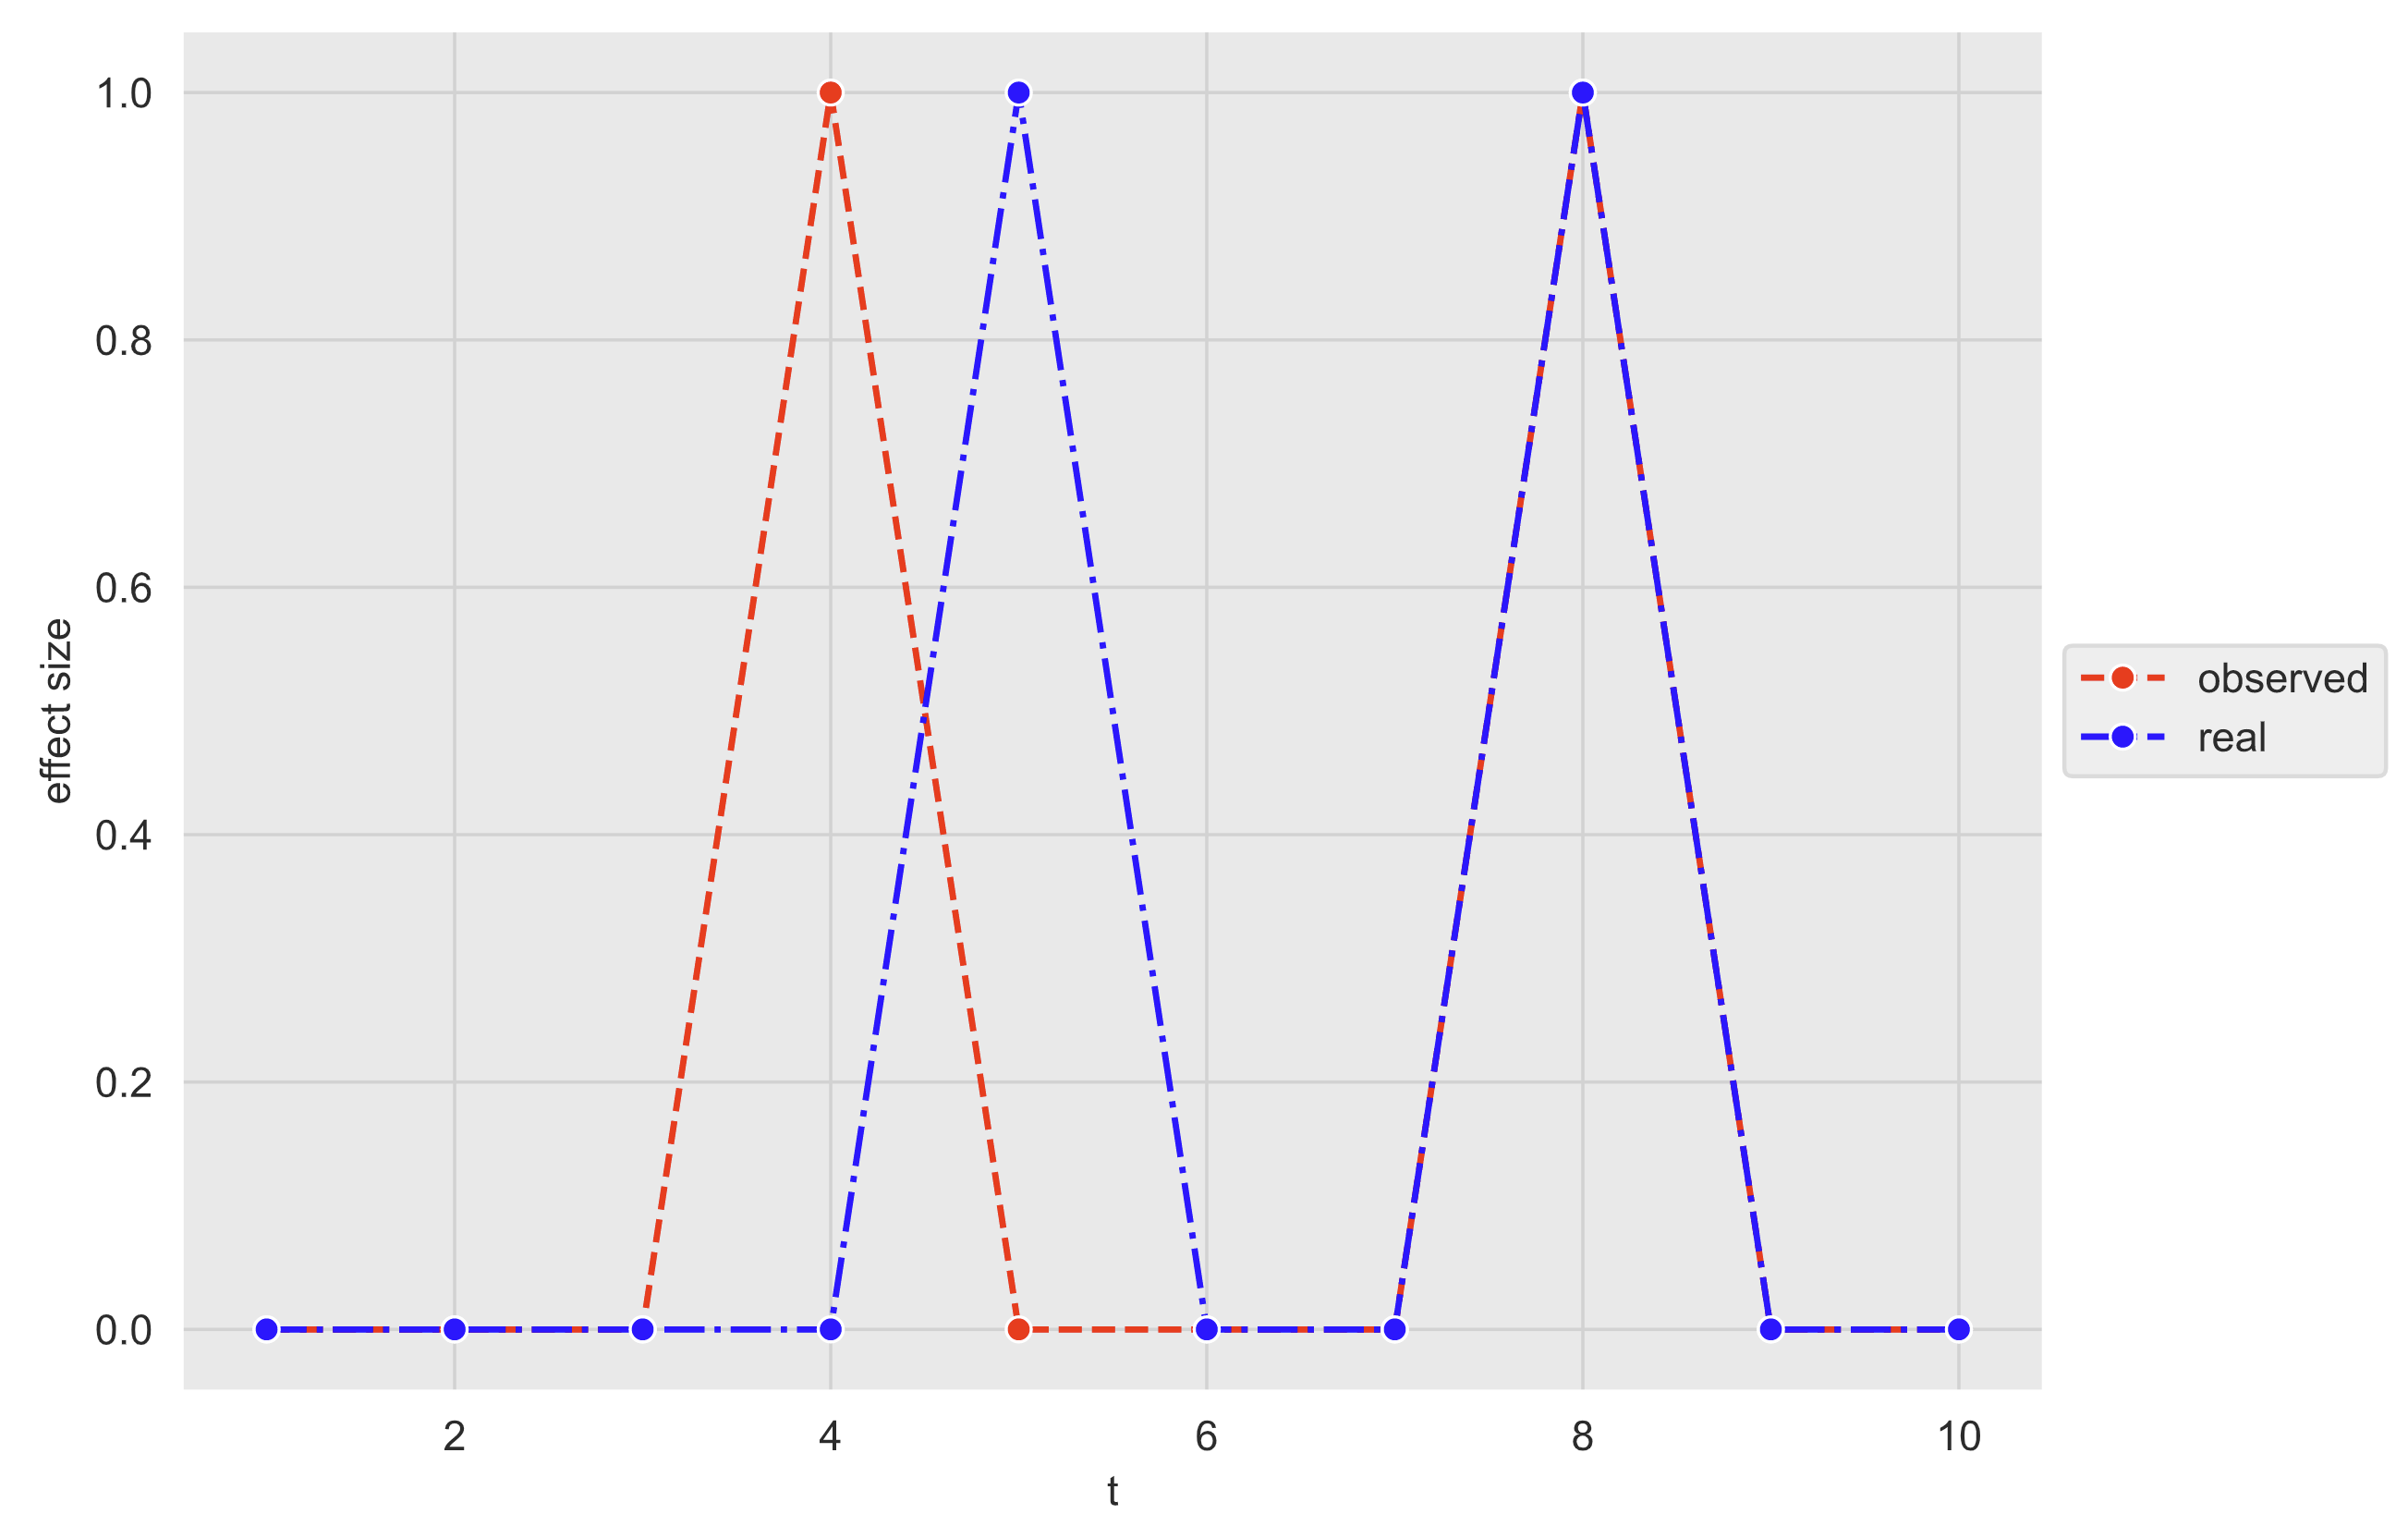
\includegraphics[totalheight=6cm]{images/2_input_delay_example.png}
\caption{Add figure caption}
\label{fig:verticalcell}
\end{figure}
\end{center}

If one were to model the effect using a fixed time delay and OLS, the estimate would only be half the true value because only one of the outputs is aligned. Obviously, this isn't ideal, we want the parameter estimates to be as close to the real values as possible, regardless of any noise in the lag structures. One can mitigate the problem via time aggregations, however in complicated multivariate cases, this is just not feasible.

Therefore, we propose a regression model which can handle stochastic time delay structures. We treat the stochastic time delay components as an ‘error’ in the time axis. Next, we find the maximum likelihood estimate, for a given set of parameters, considering the time error ($t$-axis) and the regression error ($y$-axis) simultaneously.


\section{Methodology}

We consider the problem as analogous to the typical error-in-variables (EIV) regression. Ordinary regression analyses (and machine learning models) define the loss function with respect to errors in the y axis only. For EIV, errors are considered in both the $y$-axis and the $x$-axis (REF). This is useful when there are measurement errors in the independent variable eg. because your physical measurements have some degree of random error. Similarly, for this problem we assume that we have errors in the $y$-axis and the $t$-axis. That is, there are random prediction errors and random errors in the time domain. 

Let $x: [a, b] \longrightarrow \mathbb{R}$ be a discrete time series with finite domain and we want to determine the injective, functional relationship $f$ to some other variable y. The series $x(t)$ must be a stationary series with a known value for the point at which $f(x(t)) = 0$.  That is, we know at which point the input series has no effect on the output (when it’s off). 

% TODO: Rewrite concrete expression of support...is it on x ot t?
\textcolor{red}{For clarity, as per convention, we use the nomenclature ‘support’ for the elements $f(x(t)) \neq 0$}. In addition, the series $x(t)$ should be sparse, in that it contains a low density of ‘non-zero’ coordinates. 

We also assume that the set of $\tau$'s, denoted $\mathcal{T}$, is not a constant, but rather a random draw from some discrete distribution (e.g. discrete gaussian, poisson etc). For the discrete gaussian kernel $\mathcal{T}\sim T(0, \sigma)$ or for the poisson distribution $\mathcal{T}\sim Pois(\lambda)$ and $\varepsilon \sim N(0, \sigma_{\varepsilon})$. 

Firstly, let us take the input series $x(t)$ and decompose it into its constituent non-zero impulse components. So, if $x(t)$ is a vector given by 

\begin{align}
x(t) = 
\left(
\begin{array}{cccccc}
0 & 0 & 1 & 0 & 1 & 0
\end{array}  
\right)
\end{align}

then we decompose the vector into a matrix 

\begin{align}
x(t) = 
\left(
\begin{array}{cccccc}
0 & 0 & 1 & 0 & 0 & 0 \\
0 & 0 & 0 & 0 & 1 & 0 
\end{array}  
\right)
\end{align}

where each impulse is treated separately. \\

Our algorithm then attempts to find the maximum likelihood estimate for the following equation:

% TODO fix notation for T
\begin{align}
y(t)= f(X(t + T)) + \varepsilon
\end{align}

where $X(t + T)$ is the time shifted series and $X(t)$ is the observed input.\\

In order to find the best estimate of $f$, we would like to find the function $f$ which maximises the joint likelihood of both Tau(?) and $\varepsilon$, the time-domain likelihood and the error likelihood respectively.

Specifically, we maximise the log-likelihood of the following relation:
% TODO: Clean this notation.
\begin{align}
\max  \left( \log \left(\mathcal{L}(\theta_{\varepsilon}, \varepsilon) \times \mathcal{L}(\theta_{\tau}, \tau)\right) \right)
\end{align}

where $\theta_{\varepsilon}$ and $\theta_{\tau}$ represent the parameters of the prediction error and time error respectively. For simplicity, assume that the tau and error distributions are independent. To begin with, the values of each individual time shift ($\tau$) are not known. In addition, the size of prediction error $\varepsilon$ can only be determined if each tau is known (because for each time shift there is a different prediction and prediction error). Therefore, our algorithm finds the best estimate of the individual time shifts in an inner optimisation, then iteratively searches for the best estimate of $f$ in an outer optimisation step. 

\section{Algorithm}

Firstly, we define a parametric form and some initial parameters to be estimated for the function $f$. For example, let's take the simple univariate linear model where the $f(x(t))$ is parameterised by $\beta$, $\sigma_{\varepsilon}$(error standard deviation)  and $\sigma_{\tau}$ (time error standard deviation). First, we initialise some starting values for each of these parameters.

Now we want to find the best possible time shift $\tau$ for each input impulse in $X(t)$. It stands to reason that the best possible time shift would be one that is not too far away from the observed impulse and also gives the best possible prediction. In this example, we can get the prediction y by simply multiplying the shifted value by its parameter $\beta$. From there we can calculate the likelihood estimate for time shift plus the prediction error.

In principle, we can then try a number of values of $\tau$ (i.e. optimise) until we maximise the likelihood for this impulse.

However, we must also consider that the impulses in $X(t)$ are not independent from each other. After shifting, it's possible that two or more effects can occur simultaneously.

This could be particularly problematic if there are multiple impulses within a short period of time, or the impulses have a distributed effect over multiple time points. 

As an example consider the series 

\begin{align}
x(t) = 
\left(
\begin{array}{cccccc}
0 & 0 & 1 & 1 & 0 & 0
\end{array}  
\right)
\end{align}

with $T= (1, 0)$ and $\beta = 1$. For this case, 

\begin{align}
X(t + T) = 
\left(
\begin{array}{cccccc}
0 & 0 & 1 & 0 & 0 & 0 \\
0 & 0 & 1 & 0 & 0 & 0 
\end{array}  
\right)
\end{align}

and the effect is therefore 
\begin{align}
y = 
\left(
\begin{array}{cccccc}
0 & 0 & 0 & 2 & 0 & 0
\end{array}  
\right)
\end{align}

We must consider the effects at the same time to accurately calculate the likelihood.

As shown above, if the impulses are not independent, then we need to consider time shifts $\tau$ at the same time. Therefore, we treat the problem of finding the best time shifts as a discrete optimisation problem.

For the optimisation step we utilise two assumptions to complete the optimisation. Firstly, smaller shifts are more likely than larger shifts (proportionate to the standard deviation of the T distribution). This means that we should explore the space of smaller shifts more often than larger shifts. Secondly, impulses close to each other are more likely to be dependent on each other,  than impulses further away. 

Therefore, we initialize the optimisation algorithm with all parameters set to the mean of the T distribution (e.g. zero for the zero mean gaussian). Then we randomly select a small number of impulses, the exact number could be specified manually as a hyperparameter, or inferred from the data by looking at the density of impulses in time. These impulses are randomly changed to a value drawn for the T distribution (proposal vector), and the likelihood (both time shift and prediction error) for the proposal is calculated. If the proposal likelihood is higher than the current maximum likelihood, then we update our initial estimate to the current best guess. This procedure is done in a loop, with the best guess of the set of T improving over time.

Lastly, we optimise over the set of parameters $\beta$, $\sigma_{\varepsilon}$ and $\sigma_{\tau}$, iteratively alternating between the time shift optimisation and the parameter optimisation. For the parameter optimisation, typical methods can be used such as gradient descent, genetic algorithms or annealing.  In our implementation we have used the differential evolution algorithm from the scipiy.optimize library (REF) in python, due to its ability to handle noisy objective functions. In order to improve convergence, we also standardize all input variables to the range 0-1.

Through optimisation, we find the best fit for the values of $\beta$, $\sigma_{\varepsilon}$ and $\sigma_{\tau}$. The accuracy of the final parameter estimate is relative to the ratio of the $y$-axis error and the effect size $\beta X(t)$. As $\sigma_{\varepsilon}/(\beta X(t))$ tends to infinity, the estimated value of $\sigma_{\tau}$ tends to zero. In the event that $\sigma_{\tau}=0$, the model becomes a ‘fixed lag’ model, and for the discrete gaussian case the parameter estimate $\beta$ tends to the standard linear regression coefficient.
On the other hand as $\sigma_{\varepsilon}/(\beta X(t))$ tends to zero, the estimated value of B(?) tends to the true value. Therefore, the method provides no guarantee on recovering the exact time shifts, instead only that we obtain an estimate equal to or better than standard regression.

\section{Limitations}

\section{Experiments}

\section{Future Work}

\section{Conclusion}

We have proposed a form of regression analysis for dealing with stochastic time delay problems. We have shown the feasibility of the approach and its performance on simulated data. The approach allows for better estimation and prediction when the input is affected by noise in the time domain. To our knowledge, the method is novel for this class of problem.


\end{document}